\section*{Discussion}

A multitude of processes contribute to spontaneous mutagenesis. One approach to establishing the relative importance of these is to use genomic heterogeneity in SNV density, which under a neutral model can be presumed to arise from the non-uniform action of factors contributing to mutation rate.  Identifying an association between candidate factors and SNV density can provide evidence of their effect on mutation.  In this paper we developed an approach of estimating the variance in SNV density conditioned on either recombination rate or on sequence context of various sizes.  We found an association between recombination and SNV density, obtaining estimates consistent with those from analyses of \textit{de novo} mutation data and associated recombination events.  Our analyses of contextual influences on SNV density demonstrated that the effect of context size differed between transition and transversion point mutations and did not always operate in a strand symmetric manner.

Our conclusions are derived using a model of mutation that is necessarily a simplification of a complex reality. We have assumed that each genomic site is associated with a specific mutation rate and that mutation events at different sites occur independently \citep[e.g.][]{Hodgkinson2009}. We stated earlier that achieving consistency with these assumptions requires some filtering of the data (see Assumptions in Materials and Methods). It is also known that mutations at different sites are not always independent due to the distinct phenomena of ectopic gene conversion \citep{harpak2017frequent} and of ``mutation clusters'' \citep{michaelson2012whole}. The assumption that each site has a fixed mutation rate is also a simplification as it is known that such mutation rates are influenced by external factors, notably parental age \citep[e.g.][]{francioli2015genome}.

\subsection*{The influence of recombination on mutation}

We investigated the relationship between recombination and SNV density by testing for an association between the average recombination rate evident in 10-kb genomic segments and the SNV density in those segments. Due to substantial auto-correlation of mutation and recombination rates between neighbouring segments (Figure \ref{fig:autocorrelation}), we derived estimates of the variance  using a linear regression model that was modified to incorporate this auto-correlation.  For all chromosomes examined, the posterior probabilities that the slope was $\leq 0$ were $\leq 10^{-4}$. This provides strong evidence of a positive correlation.

Taking the step from inferences about SNV density to inferences about mutation rate generally relies on an assumption that the ratio of the mutation rate to the probability of polymorphism is constant over all sites in a given population of genomes \citep[cf.][]{Hodgkinson2009}. On this basis, we can apply the ratio of the estimated point mutation rate in human chromosomes \citep{Jnsson_Parental_2017} to the average SNV density obtained from our data to express our above estimates for the slope in terms of the per base pair mutation rate per centimorgan. These results range from $2.17\times10^{-9}$ (chromosome 21) to $4.13\times10^{-9}$ (chromosome 17) (Table \ref{tab:supp-recomb}). However, such a constant relationship between SNV density and mutation rate applies to a neutral model of evolution that does not take account of at least two known factors: selective sweeps and GC-biased gene conversion (gBGC). Both of these factors are themselves influenced by the recombination rate in a region. Thus a number of factors potentially contribute to the relationship between recombination and SNV density. We aim to address the question of the contribution of a direct mutagenic effect of crossovers relative to other factors including selective sweeps and gBGC. Our approach using linear models incorporating ARMA distributions assists in this by providing a more accurate quantification of the overall relationship between recombination rate and SNV density.

We hypothesize that the direct mutagenic effect of recombination makes a significant contribution relative to the other identified factors. We compare our results to those of a recent study of \textit{de novo} mutations which estimated the probability of a recombination event (crossover) causing a mutation at $\hat{\rho}$=0.29\%, with a 95\% confidence interval of 0.17\%–0.47\% \citep{Arbeithuber_Crossovers_2015}. Such direct measurements by estimation of these rates from \textit{de novo} mutation studies constitute in principle a ``gold standard'', subject to experimental limits and small sample sizes. If $y$ is the average point mutation rate of the DNA sequence and $x$ is the average rate of crossovers, the proportion of the mutation rate that is directly caused by crossovers is $\frac{\rho x}{y}$. Setting $y=1.19\times10^{-8}$ \citep{jonsson2017whole} and $x=1.16\times10^{-8}$ \citep{Kong_2010}, we estimate the proportion of the mutation rate directly caused by crossovers at 0.28\%. If we ignore the effect of selective sweeps and gBGC by retaining the simplifying assumption that SNV density is a fixed multiple of the mutation rate regardless of location, we would predict that 0.28\% of SNVs are also directly caused by crossovers.  Comparing this to the last column of Supplementary Table \ref{tab:supp-recomb} we see that this estimate of 0.28\% for the proportion of mutations caused directly by crossovers  accounts for over 50\% of the proportion of additional SNVs associated with recombination rate as derived from our modified linear model. The latter quantity measures the influence of recombination by all mechanisms, thus this outcome provides empirical support for the hypothesized importance of the direct mutagenic effect of recombination.
 
Our estimates for the slope in terms of the base pair mutation rate per centimorgan are somewhat greater than the overall figure of $\sim1.5\times10^{-9}$ obtained in \citet{Hellmann_2005}. We note that \citet{Hellmann_2005} addressed the issue of spatial auto-correlation by means of the Cochrane-Orcutt correction \citep{kutner2005applied}, which is applicable to an auto-regressive (AR) model. AR models are nested within ARMA models as a special case. Our analysis of the residuals (data not shown) demonstrates that, taking the case of chromosome 1, the optimal ARMA model has a superior AIC ($\sim-184,554$) to the optimal AR model ($\sim-184,493$). On the other hand, our estimate of the probability that a single recombination event causes a mutation is very different from the estimate in  \citet{Hellmann_2005}, which was also based on a population analysis. In contrast to our approach, which addresses this relationship in terms of the intercept estimated from the linear model, Hellman's estimate was based on the slope. Specifically, the slope of the linear regression was estimated at $\sim1.5\times10^{-9}$ mutations per base pair per centimorgan, that is, every 1\% increase in the recombination rate in 1 Mb of sequence generated an additional $\sim0.0015$ mutations per Mb. The number of mutation events per recombination event is then taken as $0.0015/0.01=0.15$, which is two orders of magnitude greater than the empirical estimates of \citet{Arbeithuber_Crossovers_2015}. This argument implicitly treats all recombination-induced mutations as having been caused by recombination events in the most recent generation. It therefore ignores recombination-induced mutations caused by recombination events in previous generations.

The use of an ARMA distribution to model the residuals, rather than fitting a conventional linear regression, made a major difference to the results. To illustrate this, we repeated the analysis using an OLSLR model (Supplementary Table \ref{tab:supp-OLSLR}). Comparing these estimates with those from the ARMA model (Supplementary Table \ref{tab:supp-recomb}) shows marked differences in all parameter values. In particular, the variance due to recombination ($\hat{\sigma }^2_{rec}$) was some orders of magnitude larger in the OLSLR model. Critically, the intercept parameter was consistently lower for the OLSLR model and as a direct result the estimation of the number of mutations per recombination event was consistently greater for the OLSLR model by a factor of around 2. As correlations are given by the square root of $R^2$ in a linear model, the discrepancies we identify raise doubts about the accuracy of estimates of correlation between recombination rates and substitution rates in studies that do not compensate for spatial auto-correlation \citep{Lercher_2002, Duret_2008, mugal2011substitution}.
%See notebook 'Mutations and recombination using OLSLR.ipynb'

Our results indicate the effect of recombination depended on mutation direction with some mutations exhibiting no association (e.g. N\textrightarrow W transversions).  This dependence on point mutation direction has been noted by other authors and our results are generally consistent with previous observations derived from substitution data \citep{Duret_2008}. In particular, the mutation types seen to be most influenced by recombination were C\textrightarrow T and G\textrightarrow A, the same types that are subject to the CpG effect.  \citet{Arbeithuber_Crossovers_2015} reported all but one of the 17 \textit{de novo} mutations found in molecules with a crossover were of one of these two types (as were the three mutations found in non-crossover controls).  A possible explanation is that recombination magnifies the CpG effect by effecting a temporary local strand separation, since the deamination of 5-methylcytosine is over 60 times more rapid in single-stranded than in double-stranded DNA \citep{ehrlich1986dna, zhang1994effect}. The finding that the relationship between SNP density and recombination rate varied between mutation directions, including the absence of a correlation for some mutation directions, has no obvious explanation in terms of selective sweeps. This provides further support for the relative significance of the direct mutagenic effect of recombination.
%Ehrlich et al. give ssDNA rate as 9.5e-10 pwr sec: Zhang et al. give dsDNA rate as 1.5e-11 per sec. 

Recombination will only contribute to variance in SNV density insofar as it occurs heterogeneously along the genome. Neither the proportion of mutation events occurring in a single generation that are caused by recombination nor the probability that a recombination event gives rise to a mutation event (both $\sim0.004$) are affected by the distribution of recombination rates along the genome. For this reason, these quantities arguably provide a better measure of the direct effect of recombination on mutation.  A comparative analysis of $\hat{\sigma }^2_{rec}$ given in Figure \ref{fig:recomb-violin} showed some difference between chromosomes, with chromosomes 9, 15, 16, 17 and 22 having a significantly higher value of $\hat{\sigma }^2_{rec}$ than the other chromosomes. One possible explanation would be that recombination rates are more heterogeneous along these chromosomes. One measure of heterogeneity is the variance of the recombination rates, which is shown in Figure \ref{fig:rcomb-bar}. We see that chromosomes 15, 16, 17 and 22 do have relatively high variance, but not significantly higher than chromosome 13, while the variance for chromosomes 18, 20 and 21 is greater than for chromosomes 15, 16 and 17. Chromosome 9, on the other hand, does not have a relatively high variance in recombination rate. Thus while variance in the recombination rate may contribute to variance in $\hat{\sigma }^2_{rec}$, the explanation appears to be more complex. The extent of segmental duplication in chromosomes may also be a factor, as it correlates significantly with $\hat{\sigma }^2_{rec}$. The autosomes with the highest rate of segmental duplication are 7, 9, 15, 16, 17 and  22 \citep{zhang2004}. As regions of segmental duplication are susceptible to ectopic gene conversion, this process may explain an increase in $\hat{\sigma }^2_{rec}$.

Another feature of Figure \ref{fig:recomb-violin} is that chromosomes 9, 15, 16, 17 and 22 also have greater spread in their posterior distributions. This is likely to result directly from the fact that the variance due to recombination ($R^2$) is greater in these cases \citep{wishart1931mean, olkin1995correlations}. 

\begin{figure}[h!]
\begin{center}
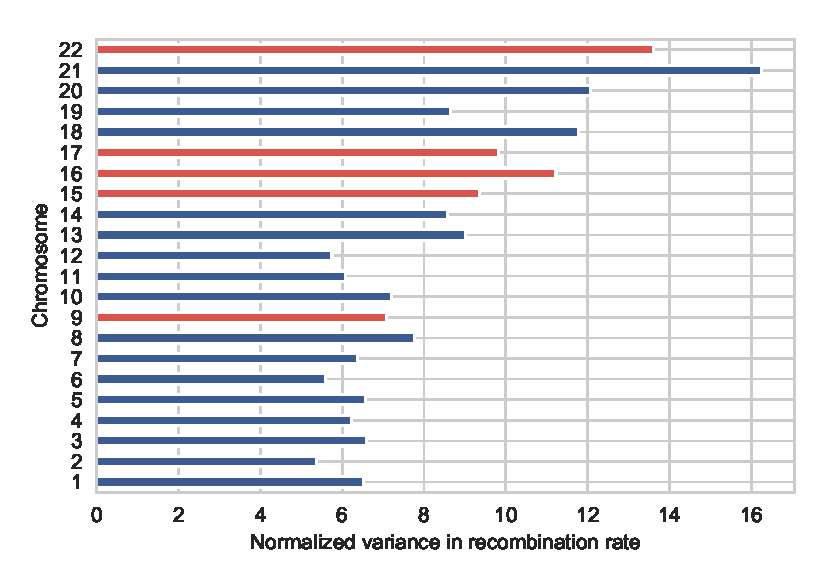
\includegraphics[width=0.5\columnwidth]{figs/recomb_bar_plot.eps}
\caption{Variance in recombination rate by chromosome. The variance in recombination rate is calculated from average recombination rates for 10-kb bins, normalized by the mean recombination rate of the entire genome.Chromosomes with a higher value of $\hat{\sigma }^2_{rec}$ are shown in red.}
\label{fig:rcomb-bar}
\end{center}
\end{figure}
 

\subsection*{The influence of context on mutation}

Our approach to analysing the influence of context on mutation has two main features: using a rich database of human variants identified by the 1KG Project \citep{Auton2015} and applying directly the concept of variance in mutation rate due to context as described in \nameref{methods}. This method is particularly suited to considering the issue of the effect on mutation of contexts of differing sizes. 

A number of authors have variously dismissed \citep{Krawczak_1998, Hodgkinson2009} or made strong claims for \citep{Aggarwala2016, Zhu_2016} the influence of contexts beyond 3-mers on mutation. Figure \ref{fig:context-var} shows that the increases from $\hat\sigma^2_3$ to $\hat\sigma^2_5$ to $\hat\sigma^2_7$ are relatively small. This is because the variance due to 3-mers incorporates the interaction between the central base of the 3-mer and its two flanking bases, which is the largest contributor to variance in SNV rates due to context. We found that $\sim54\%$ of $\hat\sigma^2_7$ was due to the CpG effect.

For analysis of an individual point mutation, the central base is fixed and thus there are no explicit interactions with neighbouring bases. In this case, which we have referred to as fixed marginals (Figure \ref{fig:context-var-individual}), the additional variance added by 5-mers over 3-mers and, to an even greater extent, by 7-mers over 5-mers is substantial.  These results may appear to support previous findings that the variance due to 7-mers is highly significant \citep{Aggarwala2016}. However, the methods used in that work differ markedly to ours.  When considering the influence of $k$-mers on the probability of observing an SNV, \citet{Aggarwala2016} fitted a linear model to binomial data, which will not yield a valid maximum likelihood estimate of the slope and intercept parameters \citep[][p. 120]{agresti}. In calculating the relative influence of 3-mers and 7-mers, they used linear regression to predict the 7-mer SNV densities from the 3-mer SNV densities and calculated the $R^2$ metric on this regression. This metric is mathematically the same as the ratio of the following quantities: sum of squares difference between the 3-mer SNV densities and the overall mean SNV density; and, the sum of squares difference between the 7-mer SNV densities and the overall mean SNV density. This ratio is in turn the ratio of variance in 3-mer SNV densities to that of 7-mer SNV densities (without being weighted by frequency of context.) This appears to account for some similarity of their results to ours.

In contrast to \citet{Aggarwala2016}, \citet{Zhu_2016} used a log-linear model for estimating the information content of neighbouring bases. This approach is appropriate in modelling binomial data and also allowed comparison of the effect of different $k$-mers as measured by information content rather than traditional sum-of-squares variance. An advantage is that the joint effect of neighbouring nucleotides can be distinguished from the independent effects of each. That work likewise identified neighbouring nucleotides as distant as 4 bases away (hence $k=9$) as associated with some transversion point mutations \citep{Zhu_2016}.

The strong influence of 7-mer contexts apparent when conditioning on the central mutating base raises the question of whether this is due to specific hyper-mutable 7-mer contexts. Our investigation failed to identify any such 7-mer contexts that were not attributable to CpG hypermutability. The most mutagenic context was NNACGNN. This sequence is of course subject to the CpG effect and the 5'-A has a positive association on C\textrightarrow T mutations independent of the 3' base \citep[see][Figure 2]{Zhu_2016}. The incidence of ACG trinucleotides was $\sim$7\% of that expected from the individual nucleotide frequencies.

Figure \ref{fig:context-sym-intronic-a} provides evidence of strand-asymmetry in the variance due to contextual influence for all 12 point mutation directions. It has been conjectured that such strand-asymmetry is caused by transcription coupled DNA repair (TCR) \citep[e.g.][]{hwang2004bayesian}. TCR is a strand-asymmetric process which occurs in actively transcribed genes when an RNA polymerase (RNAP) translocating along a DNA strand encounters a distorting lesion or other local factor that retards its forward progress and may cause it to recruit nucleotide excision repair proteins \citep{spivak2014complex}. Sequence context is known to be involved in factors that can pause or arrest RNAPs \citep{spivak2014complex}. In their phylogenetic analysis of substitution rates, \citet{hwang2004bayesian} found that T\textrightarrow C substitution rates were higher than those for A\textrightarrow G and  C\textrightarrow T substitution rates were higher than those for G\textrightarrow A. Our analysis of SNV data differs from this in showing A$\rightarrow$G to have a significantly higher SNV density than T$\rightarrow$C while C$\rightarrow$T SNVs had only marginally greater SNV density compared to G$\rightarrow$A (Table \ref{tab:supp_context}). Figure \ref{fig:context-sym-intronic-a} shows the same pattern in variance due to context: $\hat\sigma^2_7(C\rightarrow T) > \hat\sigma^2_7(G\rightarrow A)$  and $\hat\sigma^2_7(A\rightarrow G) > \hat\sigma^2_7(T\rightarrow C)$.  \citet{hwang2004bayesian} also showed transcription-associated mutational asymmetry to be influenced by context for transitions. Our results indicate that such influence occurs to some significant degree for all mutation directions. Overall, it appears that a substantial association exists between TCR and variance in SNV density.

\section*{Conclusion}

We have demonstrated that estimating the variance in SNV density due to context can discriminate the effect of contexts of different sizes. This was done from three perspectives:  considering the 12 point mutation directions separately; aggregating over these directions while marginalizing over the central allele; and aggregating over these directions without marginalizing over the central allele (measured by $\hat\sigma^2_k$). The perspective adopted has a marked influence on estimates of relative influence. For example, results aggregated over mutation direction will be dominated by the more abundant transition mutations and in particular, by the CpG effect. Our approach has clarified the relationship between results from these different perspectives and, in particular, has demonstrated the dominant effect of the interaction between a central allele and its immediate neighbours. The use of Bayesian posterior distributions was able to give a high degree of certainty to conclusions about the strand-asymmetry of contextual influence in intronic regions. Further, our methods are driven solely by varying SNV densities between contexts and are not influenced by the distribution of $k$-mers within the genome. 

We also quantified variance in SNV density due to recombination. However, a direct comparison of this quantity with the variance in SNV density due to context has some limitations. We measured variance in SNV density due to recombination at the scale of 10-kb DNA blocks. This does not take account of any variance due to recombination that exists within 10-kb blocks. This limitation is not easily overcome as there is presently no data for fine  scale recombination at the individual base level.

We note that the quantitative impacts of recombination and context on mutation are conceptually difficult to compare meaningfully, as context is a state and recombination an event. For this reason, the proportion of mutation events caused by recombination and the probability that a recombination event gives rise to a mutation event (both $\sim$0.004) are better measures of the direct impact of recombination on mutation. Our estimate that recombination only accounts for $\sim 0.4\%$ of the average mutation rate makes recombination appear a relatively minor contributor to mutation rate overall. However, recombination is concentrated in hotspots, typically 1 - 2 kb in length, in which the recombination rate can commonly be 50 or more  times higher than average \citep{international2005haplotype}.  In such regions, recombination would account for $\sim20\%$ or more of the mutation rate.